
% Define colors (ensure these are defined in your main document preamble)
\definecolor{navyblue}{rgb}{0.0, 0.0, 0.5}
\definecolor{cyan}{rgb}{0.0, 1.0, 1.0}


\section{Hypothesis and Research Goals}

\subsection{Core Hypothesis}
\begin{figure}[h!]
    \centering
    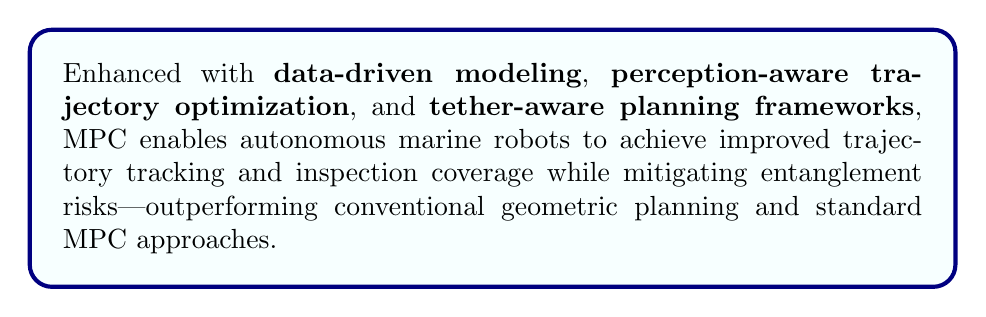
\begin{tikzpicture}[
        hypothesisbox/.style = {
            draw=navyblue,
            line width=1.5pt,
            rounded corners=8pt,
            fill=cyan!3,      % Light cyan fill
            inner sep=12pt,
            text width=0.9\textwidth,
            align=justify
        }
    ]
\node[hypothesisbox] {
Enhanced with \textbf{data-driven modeling}, \textbf{perception-aware trajectory optimization}, and \textbf{tether-aware planning frameworks}, \ac{MPC} enables autonomous marine robots to achieve improved trajectory tracking and inspection coverage while mitigating entanglement risks—outperforming conventional geometric planning and standard \ac{MPC} approaches.
};
    \end{tikzpicture}
    
    \label{fig:revised_hypothesis_separate}
\end{figure}

%what is this hypotehsis about and why did you make it?
This hypothesis proposes that three synergistic advancements to \ac{MPC} will fundamentally improve underwater inspection systems. The proposed enhancements specifically target persistent challenges in marine robotics through:

\begin{itemize}
\item \textbf{Data-Driven Modeling}: Learning complex hydrodynamic interactions that limit conventional model-based control
\item \textbf{Perception-Aware Optimization}: Actively balancing control effort with visual inspection quality during trajectory execution to ensure robust coverage.
\item \textbf{Tether-Constraints Consideration in Path planning}: Explicitly accounting for constraints that risk mission safety
\end{itemize}

\subsection{Research Goals}
The hypothesis is  be validated through focused development and testing of its constituent components:



\begin{enumerate}
\item \textbf{Design Adaptive Disturbance Learning Frameworks:}  
Implement \ac{GP} based learning to estimate environmental perturbations for MPC robustness. 

\item \textbf{Formulate a Perception-Aware \ac{MPC} Framework:}  
Integrate visual inspection quality metrics directly into MPC cost functions

\item \textbf{Design Entanglement-Aware Coverage Framework:}  
Develop real-time path planning with explicit entanglement prevention constraints

\item \textbf{Develop a Visually-Realistic Marine Robotics Simulation Platform:}  
Establish a synthetic testing environment bridging simulation-to-reality gaps
\end{enumerate}


